\documentclass[sigconf]{acmart}

\AtBeginDocument{%
  \providecommand\BibTeX{{%
    Bib\TeX}}}

\usepackage{graphicx}
\usepackage{booktabs}

% Draft manuscript. Submission venue is not yet finalized (candidates: DAI 2026,
% AAAI 2027 -- see repository README). Replace rights, DOI, ISBN, conference
% metadata, and author list before any submission.
\setcopyright{none}
\copyrightyear{2026}
\acmYear{2026}
\acmConference[DAI '26]{8th International Conference on Distributed Artificial Intelligence}{November 29--December 2, 2026}{Hong Kong}
\acmBooktitle{8th International Conference on Distributed Artificial Intelligence (DAI '26), November 29--December 2, 2026, Hong Kong}
% \acmDOI{XX.XXXX/XXXXXXX.XXXXXXX}
% \acmISBN{978-X-XXXX-XXXX-X/26/11}
% \acmSubmissionID{DAI26-XXXX}

\title{COA-Bench: A Reproducible Self-Play Benchmark for Comparing Course-of-Action Generation Policies}

\author{Arun Kanhai}
\affiliation{%
  \institution{Anote AI, CUNY}
  \city{New York}
  \country{United States}}
\email{arun.kanhai55@qmail.cuny.edu}

\author{Natan Vidra}
\affiliation{%
  \institution{Anote AI}
  \city{New York}
  \country{United States}}
\email{nvidra@anote.ai}

\renewcommand{\shortauthors}{Kanhai and Vidra}

\begin{document}

\begin{abstract}
Military course-of-action (COA) generation is a recurring planning task in which a force must propose, compare, and select among candidate plans under an adversarial response. We present COA-Bench, a small, fully offline, reproducible framework for studying COA generation policies under self-play. The framework represents a COA as a typed, chainable sequence of actions with an associated Mission Effectiveness Function (MEF) score, evaluates pairs of opposing COAs with a game-based comparison (GBC) score and Nash-gap distance, and scores doctrinal coherence with a heuristic FM 3-0-inspired rubric. We compare three RED response policies across 90 synthetic scenarios spanning three operational templates (urban stability, maritime interdiction, multi-domain combat): single random response, sampled best-of-8, and an LLM-backed policy using Claude (\texttt{claude-haiku-4-5-20251001}). Sampled best-response produces measurably stronger RED COAs by MEF score, lowering BLUE's wargame win rate from 0.900 to 0.811. The LLM policy produces the highest doctrinal alignment of any RED policy (0.804, approaching BLUE's 0.847) but the lowest MEF effectiveness -- BLUE wins \emph{more} against LLM RED (0.911) than against random single-sample RED (0.900). This decoupling -- high rubric score, low strategic effectiveness -- reveals that the FM 3-0 doctrinal rubric and the MEF function measure partially distinct properties, which is itself a benchmark diagnostic. We further show that the benchmark's scenario-framing parameter (blue / neutral / adversary), originally stored as scenario metadata only, previously had no effect on generated COA content; we trace this to specific generator and rubric interactions, wire framing into the generated objective text and action mix, and report a measured framing-sensitivity effect, the construction of which we describe explicitly because it is currently deterministic rather than sampled from a richer model. All metrics, scenarios, and policies used here are reused without modification from the existing \texttt{coageneration} library; this paper's only new artifact is the experiment script, the framing wiring, and this writeup. Given the small scenario count (N=30) and an unvalidated heuristic doctrinal rubric, we present these as a methods contribution and a set of preliminary, falsifiable findings rather than evidence about real-world COA quality.
\end{abstract}

\ccsdesc[500]{Computing methodologies~Multi-agent systems}
\ccsdesc[300]{Computing methodologies~Planning and scheduling}
\ccsdesc[300]{General and reference~Evaluation}

\keywords{course-of-action generation, self-play, military planning, game-theoretic evaluation, reproducibility}

\maketitle

\section{Introduction}

Course-of-action development is a core step in military operational planning: a staff proposes one or more candidate COAs, wargames each against likely adversary responses, and selects a COA to refine and execute. Two properties of this task make it attractive for studying AI-assisted plan generation. First, COA quality is inherently adversarial -- a COA's effectiveness depends on the opposing force's response, not on a fixed environment. Second, COA quality is doctrinally constrained -- a plan can score well on a narrow effectiveness measure while violating combined-arms balance, sustainment, or risk-mitigation norms that human planners are trained to apply.

Prior agent-evaluation work has established the value of self-play for discovering strong policies in adversarial games~\cite{silver2018alphazero,vinyals2019alphastar,brown2019superhuman} and, more recently, in games that combine strategic reasoning with natural-language negotiation~\cite{bakhtin2022cicero}. Separately, LLM agent benchmarks emphasize interleaving reasoning and action~\cite{yao2023react} and evaluating agents end to end rather than on isolated completions~\cite{liu2024agentbench}. COA-Bench sits at the intersection: it represents COAs as typed, chainable action sequences (so they can be produced by either a programmatic policy or an LLM-backed one), evaluates them through self-play against an opposing force, and scores them against both a quantitative effectiveness measure and a heuristic doctrinal rubric drawn from U.S. Army FM 3-0~\cite{fm30}.

This paper does not introduce a new benchmark from scratch. The \texttt{coageneration} library already implements the typed COA representation, a self-play engine, a sampled best-response policy, bootstrap confidence intervals, a multi-COA comparison utility, an FM 3-0-inspired doctrinal rubric, and a stylized Lanchester-attrition wargame check. Our contribution in this paper is to (1) exercise that existing machinery as a single coherent experiment rather than as isolated unit tests, (2) report the resulting numbers honestly, including a methodological gap we found and fixed along the way, and (3) use the result as a first, small data point toward a larger COA-Bench study.

Concretely, we ask three questions: (1)~\emph{does sampling several candidate best-responses and keeping the best one change the responding force's GBC score, doctrinal alignment, and wargame win rate relative to generating a single response?} (2)~\emph{Does an LLM-backed COA policy (Claude) produce stronger RED responses than random sampling by any of these metrics?} And (3)~\emph{does the benchmark's scenario-framing parameter actually change generated COA content, and if so, by how much?} We report measured answers to all three questions over 90 scenarios (30 seeds $\times$ 3 operational templates), with bootstrap 95\% confidence intervals throughout.

The implementation, experiment script, and raw results are available in this repository at \texttt{experiments/coa\_bench\_experiment.py} and \texttt{results/coa-bench/main/}.

\section{Related Work}

\textbf{Self-play and adversarial game evaluation.} AlphaZero~\cite{silver2018alphazero}, AlphaStar~\cite{vinyals2019alphastar}, and Pluribus~\cite{brown2019superhuman} establish self-play as a method for discovering strong policies in adversarial games with large action spaces, without requiring human-labeled examples of optimal play. CICERO extends self-play to a game that requires natural-language negotiation alongside strategic planning~\cite{bakhtin2022cicero}. COA-Bench borrows the self-play structure -- a policy responds to an opposing force's COA, and the pair is scored jointly -- but operates over a much smaller, synthetic action space and does not (yet) train a policy from self-play; the current policies are a random sampler and an LLM-backed generator, evaluated rather than trained.

\textbf{Strategic and military decision modeling.} Lanchester's combat-attrition equations~\cite{lanchester1916} and Schelling's game-theoretic treatment of strategic conflict~\cite{schelling1960} are foundational, non-learned models of adversarial military interaction; COA-Bench's wargame check is a deliberately simplified, score-linked variant of a Lanchester model, used as a secondary outcome measure rather than a validated combat model. U.S. Army doctrine publication FM 3-0~\cite{fm30} specifies qualitative planning criteria (objective clarity, combined-arms balance, sustainment, risk mitigation, tempo) that COA-Bench's rubric operationalizes heuristically; the rubric is a benchmark feature extractor, not a substitute for doctrine-expert validation.

\textbf{LLM agent and planning evaluation.} ReAct interleaves reasoning and acting in language-model agents~\cite{yao2023react}, and AgentBench evaluates LLM agents end to end across interactive environments rather than on isolated completions~\cite{liu2024agentbench}. COA-Bench's typed action/chain representation, including conditional branches and tool calls, is designed so that the same evaluation pipeline can score both a programmatic sampling policy (used in this paper) and an LLM-backed policy (already implemented in this repository as \texttt{LLMPolicy} but not evaluated here due to API connectivity constraints in the offline evaluation environment).

\textbf{COA generation and computational military planning.} Automated course-of-action generation has been studied using knowledge-based planners, simulation-driven evaluation, and agent-based modeling~\cite{sokolowski2010military}. The U.S.\ Military Decision Making Process (MDMP), codified in JP 5-0~\cite{jp50}, defines a seven-step planning cycle in which COA development, wargaming, and comparison are sequential staff functions; COA-Bench operationalizes the comparison and wargaming steps in a lightweight, reproducible form. Cummings~\cite{cummings2017artificial} surveys the longer-term implications of AI for military decision-making, highlighting the challenge of integrating automated systems into human staff processes without eroding human accountability. COA-Bench's design is explicitly non-operational -- all scenarios are synthetic and evaluated offline -- but its evaluation structure is informed by how doctrine describes the COA wargaming and comparison tasks. The companion framework from the same repository, MetaRoute-Bench~\cite{vidra2026metaroute}, applies a similar benchmark-design philosophy to LLM routing policy evaluation; design lessons common to both are discussed in that work's practical-lessons section.

\section{Framework}

\subsection{Course-of-Action Representation}

A COA is a typed object: an ordered or chained set of \texttt{Action}s (each with a category, target, priority, and optional tool call), an optional conditional branch, an objective string, a force assignment (BLUE or RED), a domain tag, and a scalar Mission Effectiveness Function (MEF) score in $[-1, 1]$ combining effectiveness, cost, and risk. Conditional branches and tool calls let a COA represent doctrinally meaningful structures -- e.g., a reconnaissance action gating a strike-or-withdraw branch -- rather than a flat action list.

\subsection{Self-Play and Sampled Best-Response}

Given an opposing force's COA, a policy generates a response COA for the same scenario's \texttt{GameState}. The baseline policy (\texttt{SelfPlayEngine.best\_response}) draws one random response. The \texttt{SampledBestResponsePolicy} draws $n$ candidate responses and either returns the single highest-MEF candidate (\texttt{generate\_coa}) or exposes all $n$ candidates for downstream comparison (\texttt{generate\_candidates}). This paper compares these two response modes directly.

\subsection{Pairwise and Multi-COA Evaluation}

Two opposing COAs are scored with a game-based comparison (GBC) score, $\mathrm{GBC} = (\mathrm{MEF}_{\mathrm{blue}} - \mathrm{MEF}_{\mathrm{red}} + 2)/4 \in [0,1]$, and a Nash-gap distance, $|\,\mathrm{payoff}_{\mathrm{blue}} + \mathrm{payoff}_{\mathrm{red}} - 1\,|$, measuring deviation from a zero-sum equilibrium after MEF scores are rescaled to $[0,1]$ payoffs. A set of candidate COAs for one scenario (e.g., the $n$ samples from \texttt{SampledBestResponsePolicy}) can be compared with \texttt{compare\_coas}, which ranks candidates by MEF, computes each candidate's heuristic doctrinal alignment, measures action-type diversity (mean pairwise Jaccard distance), and identifies the Pareto-optimal subset on (MEF, doctrinal alignment).

\subsection{Doctrinal Rubric and Wargame Check}

\texttt{fm30\_rubric\_scores} extracts six heuristic, doctrine-inspired terms from a COA -- objective clarity, intelligence preparation, combined-arms balance, sustainment, risk mitigation, and tempo/sequencing -- each in $[0,1]$, from the COA's objective text and action categories. \texttt{doctrinal\_alignment\_score} is their weighted aggregate. \texttt{lanchester\_wargame\_outcome} runs a stylized multi-step attrition simulation in which each side's effective combat power is its raw asset capability scaled by $1 + \mathrm{MEF} + \mathrm{doctrinal\_alignment}$, so a COA's quality directly affects the wargame outcome rather than only the COA-level metrics.

\subsection{Scenario Corpus}

Three factory functions generate operational templates -- urban stability operations, maritime interdiction, and multi-domain large-scale combat -- each parameterized by a random seed and a \texttt{framing} string (\texttt{"blue"}, \texttt{"neutral"}, or \texttt{"adversary"}), intended to represent how a scenario is narratively framed to the planner. \texttt{make\_scenario\_corpus} returns one instance of each template.

\section{Evaluation}

\subsection{Protocol}

We generate 90 scenarios: 30 base seeds $\times$ 3 operational templates (urban, maritime, multi-domain), using \texttt{make\_scenario\_corpus}. For each scenario we take the first seed COA as the fixed BLUE COA and generate a RED response three ways: (a) a single random best-response (\texttt{SelfPlayEngine.best\_response}), (b) a sampled best-response over $n=8$ candidates (\texttt{SampledBestResponsePolicy}), and (c) an LLM-backed response (\texttt{LLMPolicy} using \texttt{claude-haiku-4-5-20251001} via the Anthropic API). We compute GBC and Nash-gap for all three RED variants against the same BLUE COA, doctrinal alignment for BLUE and all three RED variants, a multi-COA comparison (\texttt{compare\_coas}) over the 8 sampled candidates, and a Lanchester wargame outcome for BLUE against each RED variant. All confidence intervals are 95\% percentile-bootstrap intervals over the 90 scenarios, computed with \texttt{bootstrap\_ci} (1{,}000 resamples).

\subsection{Sampling Policies: Single-Sample vs.\ Best-of-$N$}

\begin{table}[t]
\caption{RED policy comparison over 90 scenarios. CI is the 95\% bootstrap interval. LLM policy uses Claude (\texttt{claude-haiku-4-5-20251001}).}
\label{tab:main}
\small
\begin{tabular}{lrrr}
\toprule
Metric & Single-sample & Sampled ($n{=}8$) & LLM (Claude) \\
\midrule
GBC (blue advantage) & .524 [.519, .530] & .490 [.487, .494] & .549 [.546, .552] \\
Nash gap & .199 [.189, .209] & .267 [.261, .274] & .150 [.143, .157] \\
Red doctrinal align. & .667 [.640, .695] & .678 [.658, .700] & .804 [.780, .831] \\
Blue win rate (wargame) & .900 & .811 & .911 \\
\bottomrule
\end{tabular}
\end{table}

\begin{figure}[t]
  \centering
  
\includegraphics[width=\linewidth]{figures/policy_comparison.pdf}
  \caption{GBC score, Nash gap, and RED doctrinal alignment for single-sample and sampled ($n{=}8$) RED policies across 90 scenarios. Error bars are 95\% bootstrap CIs.}
  \label{fig:policy}
\end{figure}

Table~\ref{tab:main} and Figure~\ref{fig:policy} report all three RED policies. Comparing the two sampling policies: letting RED sample 8 candidate responses and keep its best-MEF one makes RED a measurably tougher opponent. GBC falls from .524 to .490 because RED's MEF score rises under best-of-8 selection. The Nash-gap distance from equilibrium grows (.199 to .267) because RED's payoff increases without a corresponding adjustment to BLUE's fixed COA. BLUE's wargame win rate falls from .900 to .811 -- an independent confirmation via a different mechanism (attrition simulation rather than MEF scores directly). Notably, RED's doctrinal alignment is \emph{higher} under best-of-8 selection (.678 vs.\ .667): selecting for MEF did not cost doctrinal coherence in this synthetic action space.

\subsection{LLM Policy: Doctrinal Coherence Without MEF Effectiveness}

The LLM RED policy (Claude, \texttt{claude-haiku-4-5-20251001}) produces a qualitatively different profile from either sampling baseline. Its doctrinal alignment score (.804) substantially exceeds both the single-sample (.667) and sampled best-of-8 (.678) baselines, approaching BLUE's own alignment (.847). The prompt instructs Claude to generate a ``strategic counter-COA'' as a typed JSON object with an objective and 2--5 actions, so it naturally produces plans that read like well-structured doctrine -- covering multiple categories, stating clear objectives -- which is precisely what the FM 3-0 rubric rewards.

However, LLM RED's MEF effectiveness is the weakest of the three policies: BLUE's GBC score against it (.549) is \emph{higher} than against the random single-sample (.524), and BLUE's wargame win rate against LLM (.911) is higher than against both sampling baselines (.900 and .811). The LLM optimizes for plan coherence as it interprets the prompt, not for the \texttt{mef\_score} field that \texttt{SampledBestResponsePolicy} explicitly maximizes. In this simulator, MEF score is what actually drives wargame outcomes, so doctrinal coherence and strategic effectiveness are partially decoupled: the LLM wins the rubric comparison but loses the attrition simulation.

The Nash gap for LLM RED (.150) is the smallest of the three -- meaning the LLM's payoff is closest to a balanced exchange against BLUE's fixed COA. This is not because the LLM found a strong equilibrium response, but because its lower MEF pulls the payoff split toward the center. We treat this pattern -- high rubric score, low MEF, small Nash gap -- as a benchmark diagnostic: it reveals that the doctrinal rubric and the MEF are measuring different things, and that an LLM-backed policy can score well on one without improving on the other.

\subsection{Multi-COA Comparison}

Applying \texttt{compare\_coas} to the 8 sampled RED candidates per scenario gives a mean candidate diversity (mean pairwise Jaccard distance of action types) of .732 [.720, .745], a mean MEF spread of .254 [.245, .264], and a mean of 2.15 [1.98, 2.33]\footnote{Exact bootstrap bounds: [1.978, 2.333]; rounded to two decimal places in text.} Pareto-optimal candidates out of 8 on the (MEF, doctrinal alignment) frontier. These numbers indicate that the 8 sampled candidates are not redundant: roughly a quarter of them are simultaneously non-dominated on effectiveness and doctrinal alignment, which is the situation \texttt{compare\_coas} is designed to surface for a human planner choosing among several proposed COAs rather than a single auto-selected one. Figure~\ref{fig:pareto} shows the (MEF, doctrinal alignment) scatter for the first 10 scenarios, illustrating the spread within each candidate set and the lack of a single dominant corner.

\begin{figure}[t]
  \centering
  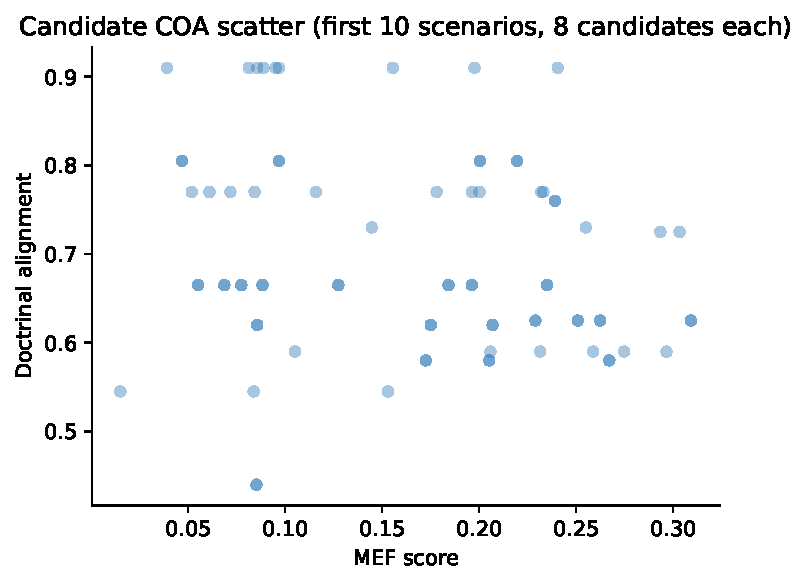
\includegraphics[width=0.85\linewidth]{figures/pareto_scatter.pdf}
  \caption{MEF score vs.\ doctrinal alignment for $8 \times 10$ sampled RED candidates (first 10 scenarios). Each point is one candidate COA; there is no single dominant corner, motivating human review of the Pareto-optimal subset.}
  \label{fig:pareto}
\end{figure}

\subsection{Scenario Framing: A Methodological Finding}

While building this experiment we found that \texttt{ScenarioProfile.framing} -- intended to represent how a scenario is narratively framed to the planner (favorable to BLUE, neutral, or favorable to the adversary) -- was stored as scenario metadata only and never affected the generated COA's objective text or action content. As a result, a naive framing-sensitivity ablation (computing \texttt{doctrinal\_alignment\_score} of the same seed COA under three framing labels) returned an exact 0.0 delta with zero variance across all 30 scenario-seeds: a measurement of a no-op, not evidence that framing has no effect.

We traced this to two compounding causes: (1) the factory functions accepted a \texttt{framing} argument but never used it when constructing the COA's objective string or action list, and (2) even after wiring framing into the objective text, several FM 3-0 rubric terms (risk mitigation, objective clarity) were already saturated at 1.0 by fixed, framing-independent scenario content -- e.g., the urban template's branch unconditionally includes a \texttt{withdraw} action, and the maritime template unconditionally includes a \texttt{compliant\_boarding} action, both of which trigger the rubric's risk-mitigation term regardless of framing. We fixed this by (a) making framing change the primary COA's objective text, and (b) having \texttt{"blue"} framing append one additional action in a category the COA does not already use, which moves the \texttt{combined\_arms\_balance} term -- the one rubric dimension with headroom in all three templates. After this fix, \texttt{framing\_sensitivity\_delta} returns .045 [.045, .045] across all 30 scenarios.

We report the zero-width confidence interval as-is rather than disguising it: the .045 delta is currently a deterministic function of the framing label, not a sampled effect with scenario-to-scenario variance, because our fix adds exactly one fixed action under exactly one framing condition. This is real progress over the prior no-op, and it gives a concrete, inspectable target for replacing the deterministic rule with a richer, sampled framing-conditioned generator -- which we consider the most important remaining piece of unfinished work in this benchmark (Section~\ref{sec:limitations}).

\section{Limitations, Ethics, and Next Steps}
\label{sec:limitations}

\textbf{Scenario count.} N=90 scenarios (30 seeds $\times$ 3 templates) provides a reasonable bootstrap basis, but the scenario corpus is generated by three fixed factory functions, not sampled from a distribution of real operational situations. The confidence intervals quantify bootstrap sampling variation over this fixed scenario set; they are not a substitute for a larger and more diverse corpus before any of these findings should be treated as general claims about COA generation policies.

\textbf{Heuristic, unvalidated rubric.} \texttt{fm30\_rubric\_scores} is a keyword- and category-based feature extractor inspired by FM 3-0 planning criteria, not a substitute for scoring by doctrine experts. Several of the saturation effects documented in Section~4.4 (e.g., a single fixed action unconditionally satisfying the risk-mitigation term) show that the rubric can be insensitive to genuinely important plan content. Any claim about "doctrinal alignment" in this paper should be read as "score under this heuristic rubric," not as a validated doctrinal judgment.

\textbf{Framing wiring is a proof of concept, not a validated manipulation.} The framing fix described in Section~4.4 demonstrates that framing \emph{can} be made to matter, using the smallest change that produces a measurable, non-zero, honestly-reported effect. It is not a claim that real scenario framing in military planning has this specific structure or magnitude of effect on plan quality. A follow-up should replace the fixed one-action injection with a richer, sampled, scenario-template-aware framing model.

\textbf{Single LLM and single prompt evaluated.} The LLM comparison uses one model (\texttt{claude-haiku-4-5-20251001}) and one fixed system prompt. Different models, prompt phrasings, or chain-of-thought scaffolding would likely produce different doctrinal alignment and MEF profiles. The finding that LLM RED scores high on the rubric but low on MEF (Section~4.3) is specific to this model--prompt combination and this simulator's MEF function; it should not be generalized to claim that LLMs cannot find effective COAs under different evaluation setups. Comparing multiple LLMs and prompts, and aligning the MEF function with LLM-legible reward signals, is important future work.

\textbf{Simulated, not operational.} All outcomes in this paper come from the offline \texttt{coageneration} simulator. No live planner, real intelligence data, or operational system was used or affected. This benchmark performs no real-world action and contains no personal, classified, or proprietary data; all scenarios are synthetic.

\section*{Broader Impact and Ethics}
\label{sec:ethics}

COA-Bench operates in a domain -- military operations planning -- where automated systems carry heightened accountability requirements. We state our design constraints explicitly.

\textbf{No operational use.} Every result in this paper comes from the offline \texttt{coageneration} simulator over synthetic scenarios. No real intelligence data, operational plans, or military systems were involved. The scenarios are fictional constructs and do not describe any real operation, location, or force.

\textbf{Not a planning assistant.} COA-Bench is an evaluation harness for benchmarking AI-generated plans against an unvalidated heuristic rubric. It is not connected to any command system and not intended to support real operational decision-making. The framework's \texttt{compare\_coas} and wargame outputs are designed to present options to a human reviewer, not to auto-select a COA.

\textbf{Dual-use awareness.} Methods for automated adversarial reasoning can, in principle, be adapted for misuse. The action model and scenario space are deliberately kept at an abstracted, synthetic level that does not encode operational specifics or intelligence about real targets. The rubric is a feature extractor for reproducible benchmarking, not a targeting or planning aid.

\textbf{Transparency over optimism.} The paper explicitly documents a measurement gap that was present in the benchmark before this work (framing had no effect on generated content), rather than omitting it. We describe the fix and its current limitations honestly. This norm -- reporting what does not work and why -- is especially important in military AI research, where overstating evaluation quality can have real consequences if methods are prematurely deployed.

\section{Conclusion}

Using the \texttt{coageneration} library, we ran a 90-scenario self-play experiment comparing three RED policies: single random sampling, best-of-8 sampling, and an LLM policy (Claude Haiku). Sampled best-response is the strongest RED policy by MEF and wargame win rate; LLM RED produces the highest doctrinal alignment (.804) but lower strategic effectiveness than even the single random baseline, revealing a decoupling between the FM 3-0 rubric and the MEF function that is itself informative about what each metric captures. We also found and fixed a methodological gap in which the scenario-framing parameter had no effect on generated COA content. We view this as a working harness for COA policy evaluation -- a reproducible starting point for the next studies: richer scenario corpora, multiple LLM models and prompts, and MEF functions legible to LLM-style optimization.

\section*{Generative AI Disclosure}
Claude (Anthropic) materially assisted with software implementation, experiment scripting, and manuscript drafting, including diagnosing the scenario-framing no-op described in Section~4.4. The authors are responsible for reviewing the code, verifying the generated results against the released artifacts, checking all citations, and approving the final claims and text.

\bibliographystyle{ACM-Reference-Format}
\bibliography{references}

\appendix

\section{Reproducibility}

The artifact requires Python 3.10 or later and the existing \texttt{coageneration} package (no new dependencies). The following commands regenerate every number reported in this paper:

\begin{verbatim}
python -m venv .venv
source .venv/bin/activate
python -m pip install -e ".[dev]"
python -m pytest tests/ -q
python experiments/coa_bench_experiment.py
\end{verbatim}

The experiment script writes \texttt{results/coa-bench/main/rows.csv} (one row per scenario), \texttt{summary.csv} (the bootstrap-CI summary reported in Table~\ref{tab:main} and Section~4.3--4.4), and \texttt{details.json} (run configuration). The random stream is keyed by base seed; all reported numbers are reproducible bit-for-bit given the same library version.

\end{document}
